
\section{Zielsetzung}
Ziel des Versuchs ist die Bestimmung unbekannter Brennweiten.

\section{Theorie}
Trifft Licht auf eine Linse wird dieses gebrochen.
Man unterscheidet zwischen Sammel- und Zerstreuungslinsen.
Sammellinsen bündeln paralleles Licht und es entsteht ein reelles Bild.
Die Brennweite und die Bildweite sind hierbei positiv.
Eine Sammellinse ist in Abbildung (\ref{fig:sam}) zu sehen.

\begin{figure}
\centering
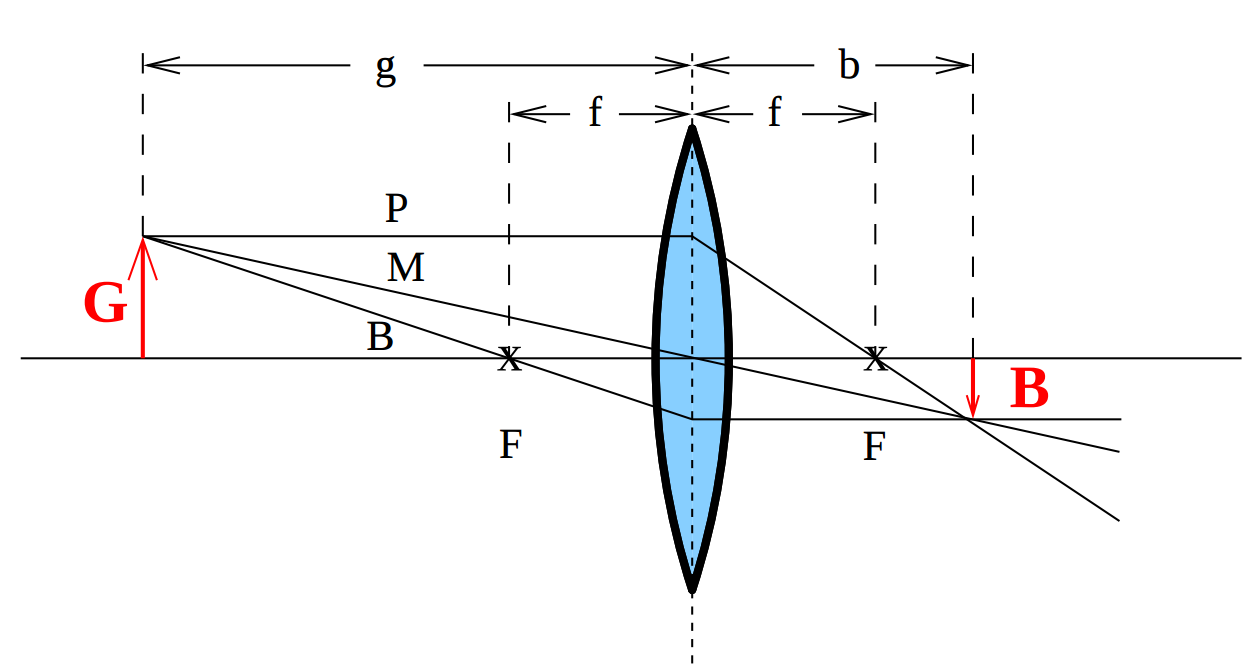
\includegraphics[height=4.60cm]{sammellinse.png}
\caption{Die Sammellinse}\cite{on1}
\label{fig:sam}
\end{figure}

Bei der Zerstreuungslinse sind Brenn- und Bildweite negativ,
sodass ein virtuelles Bild entsteht.
Sie ist in abbildung (\ref{fig:zer}) zu sehen.


\begin{figure}
\centering
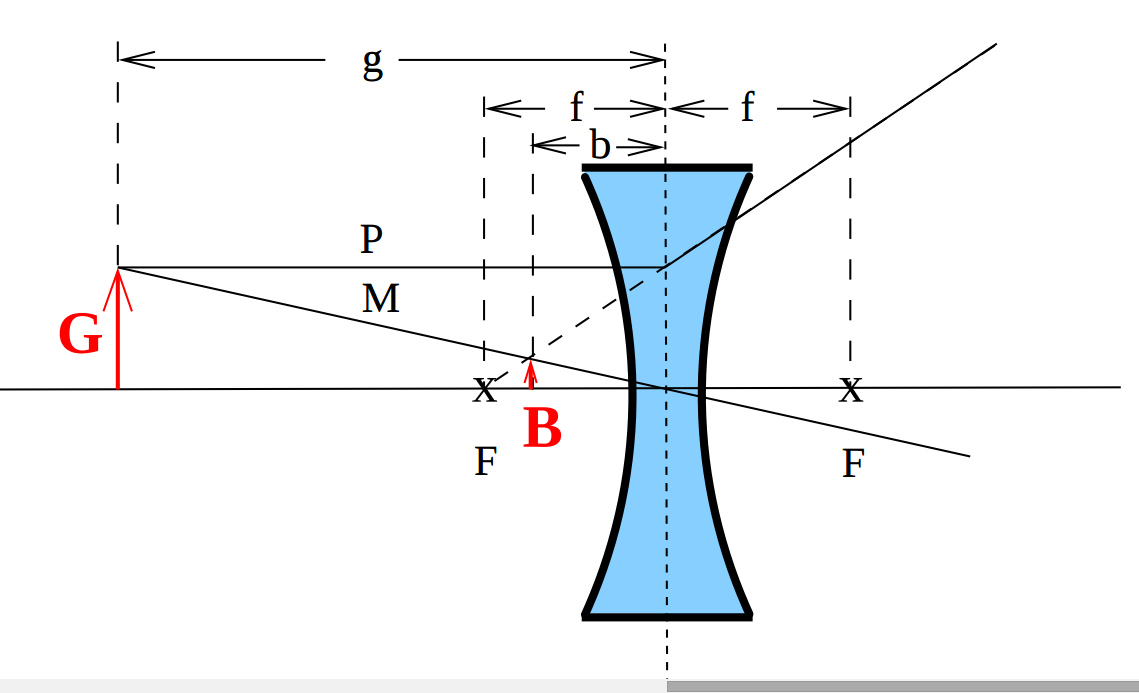
\includegraphics[height=4.60cm]{zerstreungslinse.png}
\caption{Die Zerstreuungslinse}\cite{on1}
\label{fig:zer}
\end{figure}

Für die Bildkonstruktion werden drei unterschiedliche Strahlen verwendet.\\
\emph{Parallelstrahl (P)}: Dieser verläuft Parallel zur optischen Achse und wird dann an
der Mittelebene so gebrochen, dass er durch den Brennpunkt verläuft.\\
\emph{Brennpunktstrahl (B)}: Dieser verläuft umgekehrt zum Parallelstrahl.
Er verläuft zunächst durch den Brennpunkt zur Mittelebene der Linse
und wird dann so gebrochen, dass er parallel zur optischen Achse verläuft.\\
\emph{Mittelpunktstrahl (M)}: Dieser Strahl verläuft direkt durch die Mitte,
also durch den Schnittpunkt zwischen der optischen Achse und der Mittelpunktebene.
Er wird nicht gebrochen.

Das Abbildungsgesezt
\begin{equation}
  V = \frac{B}{G}=\frac{b}{g}
  \label{eqn:abbgesetz}
\end{equation}
ergibt sich aus den Strahlensätzen und der Bildkonstruktion.
Hierbei ist V der Abbildungsmaßstab, B und G die Bild- bzw. Gegenstandsgröße und
b und g die Bild- bzw. Gegenstandsweite.
Aus dem Abbildungsgesetz folgt auch die Linsengeichung:
\begin{equation}
  \frac{1}{f}= \frac{1}{b}+\frac{1}{g}
  \label{eqn:linsgl}
\end{equation}
\subsubsection{Bestimmung der Brennweite nach der Methode von Bessel}
Bei der Methode von Bessel werden die Beiden Linsenpositionen gesucht,
an denen das Bild scharf abgebildet wird.
Dies geschieht bei konstantem Abstand zwischen Bild und Gegenstand.
Die Brennweite ergibt sich mit der Formel
\begin{equation}
  f = \frac{e^2 - d^2}{4e} .
  \label{eqn:fe}
\end{equation}
Hierbei ist e der Abstand zwischen Bild und Gegenstand und d der Abstand zwischen den beiden Lisenositionen.
Für d gilt:
\begin{equation}
  d= g_1-b_1 = g_2-b_2
  \label{eqn:d}
\end{equation}
\subsubsection{Bestimmung der Brennweite nach Abbe }
Bei der Brennweitenbestimmung nach Abbe sind zwei Linsen hintereinander angebracht.
Darum muss eine Hauptebene eingeführt werden, an der der Strah gebrochen wird.
Dies h und die Brennweite f bestimmt sich durch Formel
\begin{equation*}
  g' = g+h = f \cdot \left(1 + \frac{1}{V}\right)+h
\end{equation*}
bzw.
\begin{equation}
  b' = b+h'= f\cdot(1+V) +h'
\end{equation}
\section{Durchführung}

Die Apparatur besteht aus einer Lichtquelle und einer Schiene.
Auf der Schiene ist ein Schirm befestigt, auf dem das Bild abgebildet wird,
und eine Befestigungsvorrichtung zum Einsetzen der Linsen. Der Gegenstand,
der abgebildet werden soll, ist ebenfall auf der Schiene befestigt.
Er besteht aus einer schwarzen Scheibe mit lichtdurchlässigen Löchern, die ein 'L' ergeben.

Im ersten Teil des Veruchs wurde eine Sammellinse in der Apparatur befestigt.
Der Abstand zwischen Lichtquelle und Gegenstand wird notiert und konstant gehalten.
Die Sammellinse wird nun auf zehn unterschiedliche Entfernungen zum Gegenstand gebracht.
Zu jedem Abstand wird geguckt,
bei welcher Entfernung des Schirms zur Sammellinse das Bild scharf dargestellt wird.
Diese Messung wird für zwei unterschiedliche Sammellinsen durchgeführt.

Im zweiten Teil des Versuchs wird ebenfalls eine Sammellinse benötigt.
Die Bestimmung der Brennweite erfolgt nach der Methode von Bessel.
Der abzubildende Gegenstand wird wieder auf einem konstanten Abstand zur Lichtquelle gehalten.
Das Bild bei dieser Messung ebenfalls.
Es werden die beiden Linsenpositionen gesucht, bei der ein scharfes Bild entsteht.
Danach wird eine rot bzw. blaue Scheibe am Gegenstand befestigt.
Die Messung wird für beide Farben fünf mal wiederholt.

Im letzten Teil des Versuchs wurde nun eine Zerstreuunglinse vor der Sammellinse befestigt.
Dies ist in Abbildung (\ref{fig:linsys}) zu sehen.
Die Messung erfolgt nach der Methode von Abbe
Die Durchführung ähnelt der des ersten Teils.
\begin{figure}
\centering
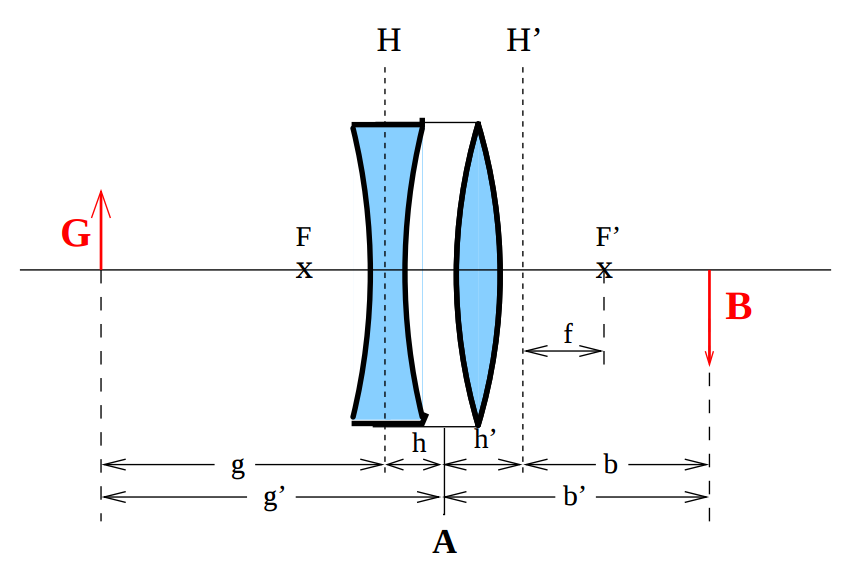
\includegraphics[height=4.60cm]{linsensystem.png}
\caption{Das Linsensystem}\cite{on1}
\label{fig:linsys}
\end{figure}
